\section{Method: changes in the book around an execution}
\label{sec:model}
Throughout this section, we consider a fixed execution and its associated participant and instrument. We omit indices identifying these objects whenever no ambiguity arises. The analysis uses the first ten occupied price levels on each side of the order book. We retain the execution index $c$ when comparing executions and the horizon $H$ when changing the observation window. All order-level quantities refer to a fixed age policy unless stated otherwise.

\subsection{Economic intuition}
A participant displays liquidity, executes on the opposite side, and withdraws previously displayed orders. Under the spoofing hypothesis, the display supports the opposite-side trade before being removed. Ordinary liquidity management can produce the same sequence: a participant may withdraw exposed orders after its inventory or market conditions change. The question is therefore not simply whether cancellation follows a trade, but how substantial the removal is and what happens to the participant's remaining display.

We answer these questions with two distinct diagnostics. The withdrawal score measures the economic scale of the initial display and its removal relative to execution and available market depth. The profile diagnostic measures the largest positive change in the participant's liquidity profile shift over a short interval following execution. Following initial orders establishes gross cancellation; following the whole profile reveals whether replacement and rebalancing maintain displayed liquidity. Their joint use corroborates the reconstructed sequence without requiring the measurements to be statistically independent. These measurements are not combined into another score. Figure~\ref{fig:topn_spoofing_timeline} illustrates the sale sequence; reversing the sides gives the corresponding purchase sequence.

% The schematic is kept in the main source immediately after this subsection.
\begin{figure}[htbp]
    \centering
    \resizebox{0.95\textwidth}{!}{%
    \begin{tikzpicture}[
        x=0.95cm,
        y=0.95cm,
        font=\small,
        book/.style={->, very thick},
        quote/.style={very thick},
        bid/.style={green!65!black},
        ask/.style={orange!85!black},
        fake/.style={fill=green!70!black, draw=green!70!black},
        real/.style={fill=red!80!black, draw=red!80!black},
        layer/.style={draw=black!45, fill=gray!8, rounded corners=2pt, minimum width=0.40cm},
        dist/.style={<->, black!70, very thick}
    ]
        \foreach \xshift/\step in {0/State 1: posturing,7.0/State 2: execution,14.0/State 3: cancellation} {
            \node[font=\large\bfseries] at (\xshift+3.0,3.15) {\step};
            \draw[book] (\xshift,0) -- (\xshift+6.0,0);
            \draw[quote,bid] (\xshift+2.25,-0.12) -- (\xshift+2.25,0.12)
                node[below=0.08cm, align=center, font=\scriptsize\bfseries] {best\\bid};
            \draw[quote] (\xshift+3.00,-0.10) -- (\xshift+3.00,0.10)
                node[above=0.10cm, font=\scriptsize\bfseries] {mid};
            \draw[quote,ask] (\xshift+3.85,-0.12) -- (\xshift+3.85,0.12)
                node[below=0.08cm, align=center, font=\scriptsize\bfseries] {best\\ask};
        }

        % State 1: layered bid-side deceptive profile and small ask-side bona fide order.
        \foreach \x/\h/\lab in {0.75/1.10/{$V_{4,b}$},1.10/1.55/{$V_{3,b}$},1.45/1.85/{$V_{2,b}$},1.80/0.45/{$V_{1,b}$}} {
            \draw[fake] (\x,0) rectangle +(0.24,\h);
            \node[above, font=\scriptsize] at (\x+0.12,\h+0.05) {\lab};
        }
        \draw[real] (4.22,0) rectangle +(0.24,0.45);
        \node[right, font=\scriptsize] at (4.48,0.30) {$V_{1,a}$};
        \node[align=center, font=\scriptsize] at (0.85,2.55) {large opposite-side\\top-ten profile};
        \node[align=center, font=\scriptsize] at (4.70,1.15) {smaller execution-side\\order};

        % State 2.
        \foreach \x/\h in {7.75/1.10,8.10/1.55,8.45/1.85,8.80/0.45} {
            \draw[fake] (\x,0) rectangle +(0.24,\h);
        }
        \draw[real] (11.22,0) rectangle +(0.24,0.45);
        \draw[orange!85!black, very thick] (11.12,0.06) -- (11.55,0.50);
        \draw[orange!85!black, very thick] (11.55,0.06) -- (11.12,0.50);


        % State 3.
        \foreach \x/\h in {14.75/1.10,15.10/1.55,15.45/1.85,15.80/0.45} {
            \draw[fake] (\x,0) rectangle +(0.24,\h);
        }
        \draw[black, very thick] (14.60,0.05) -- (16.20,1.95);
        \draw[black, very thick] (16.20,0.05) -- (14.60,1.95);


        \draw[-{Latex[length=3mm]}, thick, black!75] (6.2,1.4) -- (6.8,1.4);
        \draw[-{Latex[length=3mm]}, thick, black!75] (13.2,1.4) -- (13.8,1.4);
    \end{tikzpicture}%
    }
    \caption{Schematic top-ten timeline for the hypothesized spoofing mechanism. The large candidate posture forms an
    participant-specific depth profile over several bid levels, while the smaller order rests near the opposite best quote. The
    construction applies symmetrically to candidate buy- and sell-intent episodes. The figure shows the passive execution
    route; the operational reconstruction also admits an aggressive execution by the same actor.}
    \label{fig:topn_spoofing_timeline}
\end{figure}
\FloatBarrier



\subsection{The participant's liquidity profile}
\label{sec:spoofer_timeline}
\label{subsec:topn_depth_profiles}
By a liquidity profile we mean the participant's display across sides and price levels. The same quantity can represent a large presence in a thin book and a small presence in a deep one. We therefore compare participant quantity with total market depth at each occupied rank, then combine the shares using calibrated importance weights:
\begin{equation}
    \ell_s(t)=\sum_{k=1}^{10}w_{k,s}\frac{V_{k,s}(t)}{D_{k,s}(t)},
    \qquad s\in\{b,a\}.
    \label{eq:weighted_topn_liquidity}
\end{equation}
Here $V_{k,s}(t)$ is the participant's displayed quantity at rank $k$ on side $s$, $D_{k,s}(t)$ is total displayed market depth at that rank and side, and $w_{k,s}$ is its nonnegative calibrated weight. Rank one is the best quote; $b$ denotes bid and $a$ ask. A zero-depth level contributes zero, as specified in Appendix~\ref{sec:depth_calibration}; missing inputs are not made valid by that convention. Weights sum to one separately on each side and remain fixed within each instrument.

The weights reflect the trade-off between visibility and fill probability that motivates the hypothesized display. Under the spoofing hypothesis, an order must be visible to other participants while remaining unlikely to execute. We represent visibility through the strength of the association between a level's relative market depth and subsequent midprice movements. We represent exposure to execution by how often subsequent trades reach that level's snapshot price. A level receives greater weight when its price association is stronger and its price is less frequently reached. These are descriptive proxies: visibility is not a direct measurement of attention or causal price impact, and price-reaching frequency is not the fill probability of an individual order, which also depends on queue position and intervening events.

The calibrated weights differ across ranks, book sides, and instruments. Table~\ref{tab:empirical_depth_kernel_calibration} retains the side-specific estimates used in the calculations. Figure~\ref{fig:empirical_top10_kernel_profiles} summarizes their arithmetic average across sides for visualization; Figures~\ref{fig:empirical_topn_visibility_profiles} and~\ref{fig:empirical_topn_execution_risk_profiles} show the visibility proxy and price-reaching frequencies underlying the trade-off. Calibration uses $H_{\mathrm{cal}}=1$ second throughout, including when participant behavior is followed for longer. Appendix~\ref{sec:depth_calibration} gives the estimation procedure, normalization, and uncertainty calculations. The weights use the full sample of each instrument; prospective evaluation would require estimation on earlier data.

\begin{table}[htbp]
\centering
\caption{Full-sample empirical top-$10$ depth-kernel weights recalibrated at horizon $H_{\mathrm{cal}}=1$ second. Values are rounded to
three decimal places and sum to one within each instrument and side before rounding.}
\label{tab:empirical_depth_kernel_calibration}
\small
\setlength{\tabcolsep}{3pt}
\begin{tabular}{ll*{10}{r}}
\toprule
Instrument & Side & $\widehat w_1$ & $\widehat w_2$ & $\widehat w_3$ & $\widehat w_4$ & $\widehat w_5$ & $\widehat w_6$ & $\widehat w_7$ & $\widehat w_8$ & $\widehat w_9$ & $\widehat w_{10}$ \\
\midrule
Risanamento & Ask & 0.108 & 0.263 & 0.362 & 0.011 & 0.016 & 0.043 & 0.000 & 0.019 & 0.104 & 0.073 \\
 & Bid & 0.645 & 0.036 & 0.024 & 0.148 & 0.053 & 0.023 & 0.019 & 0.037 & 0.014 & 0.002 \\
Nexi & Ask & 0.103 & 0.023 & 0.021 & 0.177 & 0.253 & 0.052 & 0.315 & 0.019 & 0.006 & 0.032 \\
 & Bid & 0.073 & 0.131 & 0.104 & 0.208 & 0.223 & 0.120 & 0.028 & 0.030 & 0.004 & 0.078 \\
Ferrari & Ask & 0.060 & 0.040 & 0.053 & 0.277 & 0.349 & 0.023 & 0.163 & 0.012 & 0.002 & 0.022 \\
 & Bid & 0.154 & 0.095 & 0.023 & 0.103 & 0.116 & 0.248 & 0.005 & 0.071 & 0.114 & 0.070 \\
\bottomrule
\end{tabular}
\end{table}

\input{generated/simple_notation_20261020/kernel_figures.tex}
\FloatBarrier

To distinguish ask-dominated from bid-dominated display, we use the liquidity imbalance:
\begin{equation}
    I(t)=\begin{cases}
        \dfrac{\ell_a(t)-\ell_b(t)}{\ell_a(t)+\ell_b(t)},
            &\ell_a(t)+\ell_b(t)>0,\\[4pt]
        \text{undefined},&\ell_a(t)+\ell_b(t)=0.
    \end{cases}
    \label{eq:multilevel_dwi}
\end{equation}
When defined, $I$ lies in $[-1,1]$. Positive values indicate ask-side dominance and negative values bid-side dominance. Values near zero indicate approximately balanced weighted shares only when liquidity is present. The reconstructed series records zero once to mark disappearance of a previously observed profile; other undefined values remain missing. That marker is not evidence of renewed balance. Figure~\ref{fig:topn_imbalance_dynamics} illustrates the economic contrast, not an empirical classification rule.

\begin{figure}[htbp]
    \centering
    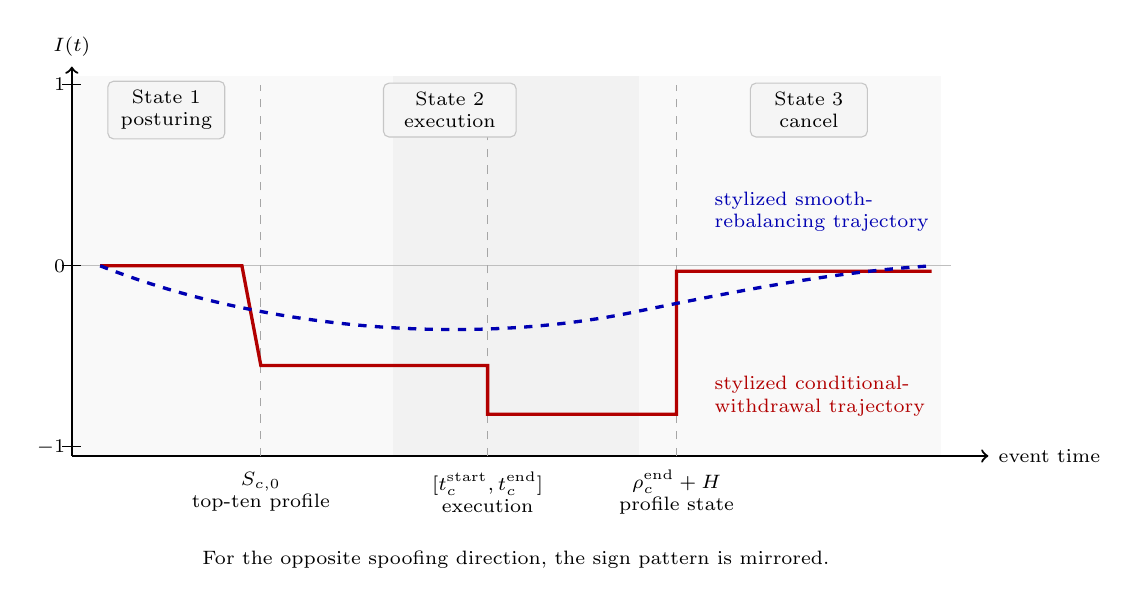
\begin{tikzpicture}[
        x=2.4cm,
        y=2.3cm,
        font=\scriptsize,
        axis/.style={->, thick},
        spoof/.style={very thick, red!70!black},
        maker/.style={very thick, dashed, blue!70!black},
        event/.style={gray!70, dashed},
        state/.style={fill=gray!8, draw=gray!45, rounded corners=2pt, align=center}
    ]
        \fill[gray!5] (0,-1.05) rectangle (1.7,1.05);
        \fill[gray!10] (1.7,-1.05) rectangle (3.0,1.05);
        \fill[gray!5] (3.0,-1.05) rectangle (4.6,1.05);

        \draw[axis] (0,-1.05) -- (0,1.1) node[above] {$I(t)$};
        \draw[axis] (0,-1.05) -- (4.85,-1.05) node[right] {event time};
        \draw[gray!50] (-0.05,0) -- (4.65,0);

        \foreach \y/\lab in {-1/$-1$,0/$0$,1/$1$} {
            \draw (-0.05,\y) -- (0.05,\y) node[left=0.08cm] {\lab};
        }

        \draw[event] (1.0,-1.05) -- (1.0,1.0);
        \draw[event] (2.2,-1.05) -- (2.2,1.0);
        \draw[event] (3.2,-1.05) -- (3.2,1.0);

        \node[state, text width=1.25cm] at (0.5,0.86) {State 1\\posturing};
        \node[state, text width=1.45cm] at (2.0,0.86) {State 2\\execution};
        \node[state, text width=1.25cm] at (3.9,0.86) {State 3\\cancel};

        \node[align=center] at (1.0,-1.25) {$S_{c,0}$\\top-ten profile};
        \node[align=center] at (2.2,-1.25) {$[t_c^{\mathrm{start}},t_c^{\mathrm{end}}]$\\execution};
        \node[align=center] at (3.2,-1.25) {$\rho_c^{\mathrm{end}}+H$\\profile state};

        \draw[spoof] (0.15,0) -- (0.9,0)
            -- (1.0,-0.55) -- (2.2,-0.55)
            -- (2.2,-0.82) -- (3.2,-0.82)
            -- (3.2,-0.03) -- (4.55,-0.03);

        \draw[maker] (0.15,0) .. controls (1.0,-0.35) and (2.1,-0.45) .. (3.0,-0.25)
            .. controls (3.7,-0.10) and (4.1,-0.03) .. (4.55,0);

        \node[red!70!black, align=left, anchor=west] at (3.35,-0.72) {stylized conditional-\\withdrawal trajectory};
        \node[blue!70!black, align=left, anchor=west] at (3.35,0.30) {stylized smooth-\\rebalancing trajectory};
        \node[align=center] at (2.35,-1.62) {For the opposite spoofing direction, the sign pattern is mirrored.};
    \end{tikzpicture}
    \caption{Stylized execution-time behavior of the liquidity imbalance. The conditional-withdrawal
    trajectory shows a large top-ten imbalance returning rapidly toward zero after the opposite-side execution. The smooth
    trajectory illustrates gradual rebalancing. Neither trajectory is an empirical classification rule.}
    \label{fig:topn_imbalance_dynamics}
\end{figure}
\FloatBarrier



\subsection{Changes in the liquidity profile}
\label{subsec:multilevel_conditionality}
\label{subsec:msci_grid_method}
An imbalance change alone does not identify which side recedes. For a sale, withdrawal of the hypothesized display occurs on the bid side; for a purchase, it occurs on the ask side. Let $s$ denote the execution side and $\bar s$ its opposite. We measure each side's proportional reduction from its pre-execution weighted share:
\begin{equation}
    r_s(H)=\begin{cases}
        \dfrac{[\ell_s(t_c^-)-\ell_s(t_c^+)]_+}{\ell_s(t_c^-)},
            &\ell_s(t_c^-)>0,\\[4pt]
        0,&\ell_s(t_c^-)=0.
    \end{cases}
    \label{eq:side_collapse}
\end{equation}
Here $[x]_+=\max\{x,0\}$. The state $t_c^-$ is the last retained participant state before the first execution message. The state $t_c^+$ depends on $H$: it is the last supported retained state at or before $H$ seconds after the final execution message's sequence time. These labels identify selected book states, not new trade timestamps. Missing required states leave profile changes missing. Appendix~\ref{sec:profile_technical} specifies observation support and evaluation of the zero-initial-liquidity branch.

A directional profile shift combines the magnitude of imbalance change with the difference between the two reductions:
\begin{equation}
    \Phi_c(H)=\frac12\left|I(t_c^+)-I(t_c^-)\right|
                 +r_{\bar s}(H)-r_s(H).
    \label{eq:signed_msci}
\end{equation}
The first component measures imbalance change, scaled to $[0,1]$; the second increases the shift when opposite-side liquidity recedes; the third offsets execution-side recession. The shift lies in $[-1,2]$ when defined, without clipping. It is an intermediate description of profile change, not another ranking score. Fills, replacement orders, changes in rank, and other participants' depth can change the weighted shares without cancellation of the initial orders.

To locate a sharp transition rather than only an endpoint difference, we evaluate the same shift throughout the window, always keeping the pre-execution baseline fixed. Its largest positive increment over a 50-millisecond interval is
\begin{equation}
    J_c(H)=\max_k\left[\Phi_c(u_k)-\Phi_c(u_{k-\lambda})\right]_+.
    \label{eq:msci_grid_increment}
\end{equation}
The elapsed-time grid has 10-millisecond spacing, includes both endpoints of $[0,H]$, and compares nodes five steps apart ($\lambda=5$). Here $\Phi_c(u)$ evaluates the shift at elapsed sequence time $u$, always against the same pre-execution profile. We use $H\in\{1,2,5,10\}$ seconds, with ten seconds primary. The complete grid definition, canonical message ordering, forward carry of retained states, missing-profile rules, and maximizing-interval ties are in Appendix~\ref{sec:profile_technical}.

A large $J$ indicates a sharp positive profile-shift change, not spoofing or speed independently of amplitude. A persistent and a temporary increase can have the same $J$; a constant trajectory has $J=0$, but $J=0$ does not imply an unchanged profile. Incomplete trajectories remain missing rather than zero. The profile includes every displayed order at the first ten levels, irrespective of age, so $J$ does not change across age policies for a fixed execution and horizon. It neither selects candidates nor determines the withdrawal-score ranking.

\subsection{Withdrawal and market relevance}
\label{subsec:withdrawal_market_age}
To establish actual withdrawal, we fix the participant's opposite-side orders present within the first ten market levels immediately before execution. Their initial quantity is $P_c$; later submissions do not enter this display. The execution quantity is $Q_c>0$, and $U_c(H)$ is the physical quantity withdrawn through assigned cancellations within the horizon. Finally, $D_c$ is total opposite-side market depth over those ten levels in the exact pre-execution book, including the participant's orders. This denominator stays fixed rather than following later market depth.

The ratios $U_c(H)/Q_c$ and $U_c(H)/P_c$ answer different questions: how much is withdrawn relative to execution, and how much of the initial display disappears? The latter lies in $[0,1]$ when $P_c>0$ and is undefined when $P_c=0$. No assigned cancellation gives $U_c(H)=0$. Withdrawal is gross removal: replacement orders are not subtracted. Initial-order caps prevent repeated cancellations or later size increases from inflating removal, and assignment is exclusive within each horizon and age setting. Appendix~\ref{sec:withdrawal_technical} gives the complete physical accounting.

Observation of withdrawal starts from the final execution trade time, whereas profile observation starts from its final message's sequence time. Withdrawal includes nonnegative cancellation delays strictly below $H$ and requires source-order precedence. These clocks have an operationally assumed common origin, not independently certified synchronization; all comparisons retain integer nanoseconds (Appendix~\ref{sec:data_details}).

An older visible order remains eligible in the main specification, but receives less weight in the score. For initial order age $a$, the main weight is
\begin{equation}
    g(a)=2^{-a/(30\,\mathrm{s})}.
    \label{eq:shared_order_age_weight}
\end{equation}
The weight halves every 30 seconds. Age is measured from the lifecycle's first observed sequence time to the first execution message and frozen there. The same frozen weight multiplies the initial displayed quantity and its subsequent counted cancellation, giving $P_c^{\mathrm{age}}$ and $U_c^{\mathrm{age}}(H)$. Only initial order age is discounted: there is no cancellation-delay discount. Neither $Q_c$, $D_c$, nor the complete liquidity profile is age-discounted. The 30-second half-life is an exploratory specification, not a fitted behavioral constant. Full sums, lifecycle conventions, and alternative policies are given in Appendix~\ref{sec:withdrawal_technical}.

We measure the economic scale of withdrawal with the withdrawal score:
\begin{equation}
    W_c(H)=
      \log\!\left(1+\frac{P_c^{\mathrm{age}}}{Q_c}\right)
      \log\!\left(1+\frac{U_c^{\mathrm{age}}(H)}{Q_c}\right)
      \frac{U_c^{\mathrm{age}}(H)}{D_c}.
    \label{eq:wmsci_market_age}
\end{equation}
Here $\log$ is the natural logarithm. The first factor describes initial display relative to execution; the second describes withdrawal relative to execution. Their logarithms moderate very large quantity ratios. The third factor places withdrawal relative to initial market depth. It remains linear so that, holding the logarithmic factors fixed, the score is proportional to the market share withdrawn. Multiplication emphasizes their joint presence: a small component attenuates the others, and no withdrawal gives zero. An additive score could reward display without removal unless another rule prevented it.

The score is nonnegative and has no fixed upper bound. It orders review, not manipulation probabilities. Accounting ensures $0\leq U_c^{\mathrm{age}}(H)\leq P_c^{\mathrm{age}}\leq D_c$ when depth is measured, so its final factor lies in $[0,1]$. For $Q_c>0$ and positive measured $D_c$, zero weighted display or withdrawal gives $W=0$ directly. Missing or zero $D_c$ makes the score unavailable; no artificial denominator quantity is added. Underflow of age weights or scores never removes a physical candidate. The score uses aggregate top-ten quantity, while $J$ describes rapid change in the relative profile; neither replaces the other.

\subsection{Candidate identification and review ranking}
\label{subsec:candidature_priority}
An execution is a candidate in a horizon and age setting precisely when executed quantity, eligible raw initial display, and assigned raw withdrawal are all positive. No minimum withdrawal-to-execution ratio, profile threshold, score threshold, or favorable-price condition is imposed. Every execution and parameter setting remains represented, including non-candidates, so changes in coverage can be traced.

Within each instrument and setting, candidates with finite scores are ordered by descending $W$, including zero scores at the end. Ties use stable execution identifiers, then partition and participant identifiers. Candidates without finite scores remain explicitly unranked, with a reason; missing scores are not replaced by zero. The analyst's stopping depth is a workload decision, not a boundary between manipulation and legitimate activity.

The value of $J$ accompanies the execution without filtering, reordering, or breaking ties. A small $J$ can coexist with substantial removal, and a large $J$ can precede cancellation of the initial display. Price diagnostics likewise add interpretation without changing membership or rank. Comparisons across settings retain the original execution identity: repeated views and shared physical messages are not independent evidence. Appendix~\ref{subsec:event_reconstruction} defines shared-order episodes as a contextual grouping, not another selection.

\subsection{Price diagnostics}
\label{sec:price_measures_simple}
\label{subsec:primary_price_selection}
\label{sec:joint_selection_simple}
The hypothesized purpose of the display is to improve an opposite-side trade. Prices therefore ask three additional questions: does the midprice move favorably before execution, does it revert after withdrawal, and how does the actual execution price compare with the completed display? These comparisons retain source price units, not ticks, and do not identify causal price effects.

Let $M(t)$ be the midprice and let $d_c=+1$ for a sale and $d_c=-1$ for a purchase, so favorable movement is positive. The completed-display benchmark $S_{c,0}$ is the saved state immediately after the last candidate order was first observed in source order. It must strictly precede the execution's first message; it is not the price before all orders were placed. Favorable price movement is
\begin{equation}
    \operatorname{FPM}_c=d_c\left[M(t_c^-)-M(S_{c,0})\right].
    \label{eq:favorable_price_move}
\end{equation}
A higher pre-execution midprice is favorable to a sale, and a lower one to a purchase. The saved state $t_c^-$ need not be the immediately adjacent global book. Missing benchmarks remain missing rather than zero.

Reversion checks the opposite direction after assigned cancellations. For each positive counted cancellation $j$, let $M_j^{\mathrm{saved}}$ be the last retained pre-cancellation midprice and $M_j^{R}$ the retained price at or before $\rho_j+H_R$, with the separate reversion horizon $H_R=2$ seconds. Using physical counted quantities $\bar q_{c,j}$, we define
\begin{equation}
    \operatorname{REV}_c=
    \frac{\sum_{j\in\mathcal C_c^+(H)}\bar q_{c,j}d_c
                [M_j^{\mathrm{saved}}-M_j^{R}]}
         {\sum_{j\in\mathcal C_c^+(H)}\bar q_{c,j}}.
    \label{eq:price_reversion}
\end{equation}
Here $\mathcal C_c^+(H)$ contains all assigned cancellations with positive counted quantity. The value is defined only when this set is nonempty and every member has both finite prices and supported observation through its target. Otherwise complete REV is missing; an observed-subset mean does not replace it. The weights are physical quantities, not age weights or cancellation-delay discounts. The retained market quotes need not be fresh at two seconds, and no maximum saved-state age is imposed. Appendix~\ref{subsec:price_response_diagnostics} specifies joins, equal-time ordering, and missing-price rules.

Finally, let $\bar p_c$ be the quantity-weighted execution price. Execution advantage is
\begin{equation}
    \operatorname{ADV}_c=d_c\left[\bar p_c-M(S_{c,0})\right].
    \label{eq:execution_advantage}
\end{equation}
Positive ADV means selling above or buying below the completed-display midprice. It is a price comparison, not realized profit, and can reflect the spread even without favorable midprice movement. Subtracting FPM gives the signed difference between execution price and the saved pre-execution midprice.

The reported prices use the main ten-second withdrawal window and 30-second age half-life; these setting arguments are suppressed in FPM, REV, and ADV. Every one of the 6,914 candidates remains in its instrument's denominator, including zero-score candidates and positive, zero, negative, or missing prices. Values within the endpoint-scale floating-point bound count as numerical zero only for sign summaries and medians, without changing raw prices or selection. Appendix~\ref{subsec:price_numerical_signs} gives this convention and its sensitivity check. Appendix~\ref{subsec:price_response_diagnostics} also retains the alternative microprice and the accounting decomposition of observed reversion, not a counterfactual market without the participant.

Table~\ref{tab:simple-terminology} collects the observational units and the distinct roles of candidature and review priority.
\begin{table}[!htbp]
\centering
\caption{Terms used in the main specification. Candidate orders need not be cancelled, whereas a candidate execution requires positive assigned withdrawal. Executions, not orders or episodes, are the unit of the main comparisons.}
\label{tab:simple-terminology}
\begin{singlespace}
\renewcommand{\arraystretch}{1.18}
\begin{tabularx}{\textwidth}{@{}>{\raggedright\arraybackslash}p{0.25\textwidth}>{\raggedright\arraybackslash}X@{}}
\toprule
Term & Meaning in this paper \\
\midrule
Message or fill & An individual source record. Related partial fills can be grouped into one execution. \\
Execution (execution cluster) & Fills of the same order grouped under the participant, role, side, partition, lifecycle, price, and time-gap rules. Called an execution after its definition. \\
Participant & The original client where identified, or a separately retained firm fallback. Firm fallback can pool several clients; it is not the complete intermediary view below. \\
Candidate orders or initial display & The participant's opposite-side orders active within the first ten market price levels immediately before execution. The main setting retains all observable nonnegative ages; later orders do not enter this display. \\
Assigned withdrawal & Cancellation of initial orders assigned exclusively to an execution within the observation window and capped at their initial quantity. This is gross removal, without subtracting replacements. \\
Candidate execution & An execution with positive executed quantity, eligible raw initial display, and assigned raw withdrawal in the stated setting. No $W$, profile, or price-sign threshold is required. \\
Withdrawal-score rank & The position obtained by ordering candidates by decreasing withdrawal score within instrument and setting. Finite zero scores remain; unavailable scores are explicitly unranked. \\
Profile diagnostic $J$ & The largest positive profile-shift increment over the specified short comparison interval. It accompanies the ranking without selecting candidates or changing their order. \\
Shared-order episode & Executions connected, directly or indirectly, through shared candidate-order lifecycles within participant, execution side, partition, and recorded date. This grouping supplies context, not a further selection. \\
Identified-client and intermediary views & Client groups use executions with an identified client. Intermediary groups use the original firm on every execution, including client-identified and firm-only activity. The views overlap and are not additive. \\
\bottomrule
\end{tabularx}
\end{singlespace}
\end{table}
\FloatBarrier


\FloatBarrier
